\chapter{Plugin Design and Architecture}

This appendix documents the design and architecture of the Boss DS-1 neural emulation plugin produced as the primary deployed artefact of this research. It covers the rationale for the chosen development framework, the constraints that govern real-time audio plugin design, the signal processing chain, the machine learning inference strategy, and the user interface implementation. A screenshot of the plugin loaded in Ableton Live 12 is shown in Figure~\ref{fig:plugin_screenshot}.

\section{Development Framework: JUCE}

The plugin was developed using JUCE (Jules' Utility Class Extensions), a C\texttt{++} framework that has become the de facto standard for professional audio plugin development~\cite{noauthor_juce-frameworkjuce_2026}. JUCE is deployed in production by a wide range of major manufacturers, including Native Instruments, Arturia, iZotope, Focusrite, and Steinberg, and underpins a substantial proportion of the commercial plugin ecosystem.

The central problem JUCE solves is one of fragmentation. The audio plugin industry does not operate on a single standard format. VST3, developed and maintained by Steinberg, is the dominant open format on both Windows and macOS. Apple's Audio Units (AU) format is required for full integration with Logic Pro and GarageBand on macOS. Avid's AAX format is mandatory for Pro Tools, which remains the standard DAW in professional post-production and broadcast facilities. Newer formats such as CLAP (CLever Audio Plug-in API) are also gaining adoption. Without an abstraction layer, supporting all of these formats requires maintaining largely separate codebases for each, because each SDK presents a different API for the same fundamental operations: receiving audio buffers, exposing parameters, saving and restoring state. Platform fragmentation compounds this further: a VST3 built for Windows requires separate code to run on macOS, and a plugin targeting embedded Linux hardware such as a Raspberry Pi represents yet another compilation target.

JUCE resolves both dimensions of this fragmentation through a unified \texttt{AudioProcessor} API. From one codebase, the framework generates standards-compliant VST3, AU, AAX, and Standalone targets across Windows, macOS, Linux, iOS, and Android, while handling the format-specific wrapper code automatically. For this research, the priority was machine learning inference and the comparative evaluation of GRU and LSTM architectures rather than commercial cross-platform release engineering. The implemented build therefore focuses on the JUCE targets used in this repository: AU, VST3, and Standalone. As reported in Chapter~4, final runtime testing was carried out in Ableton Live~12 and Cubase~12 using AU and VST3 builds.

\section{Real-Time Constraints}

Audio plugin development imposes a category of engineering constraint that does not arise in most other software contexts. The host DAW delivers audio to the plugin in fixed-size blocks --- commonly 64, 128, 256, or 512 samples, depending on the session's buffer size setting. At a sample rate of 44.1~kHz with a 128-sample buffer, the host issues a new block approximately every 2.9~milliseconds. The plugin must complete all processing for that block and return a result before the next block arrives. Failing to meet this deadline causes a buffer underrun, heard as an audible click or dropout.

Critically, the plugin does not have exclusive use of that 2.9~ms budget. The audio thread must also service every other plugin on every other track in the session, the DAW's own internal processing, and any other system processes competing for the CPU at the same moment. A single computationally expensive plugin can therefore make an entire session unusable, not only for itself but for everything running alongside it. This places a hard ceiling on per-sample computational cost that has no equivalent in offline processing contexts.

The real-time constraint imposes an equally important architectural rule: the audio processing thread must never perform dynamic memory allocation, acquire a mutex lock, or conduct file I/O. Any of these operations can stall execution for an indeterminate amount of time while the operating system services the request, producing a latency spike that registers as an audible glitch. A plugin that performs an allocation on the audio thread may work correctly in most circumstances and fail unpredictably under system load. For this reason, all resources required at runtime --- including both neural network models --- are allocated and initialised during the plugin's \texttt{prepareToPlay()} call, which occurs before the audio thread becomes active. Nothing is allocated during audio processing.

\section{Signal Chain and Neural Network Inference}

The plugin implements the following signal chain within each audio buffer callback:

\begin{enumerate}
  \item \textbf{Input gain (Drive).} The incoming audio sample is scaled by a linear gain factor derived from the Drive parameter, which is expressed in decibels and converted to a linear multiplier at parameter update time.

  \item \textbf{Mono wet-path preparation.} The model is trained for mono input and mono output. In stereo plugin configurations, the wet path therefore sums the two input channels to mono before neural inference. The processed mono output is then copied back to the plugin output channels and blended against the dry signal according to the bypass state.

  \item \textbf{Host-to-model sample-rate conversion.} The recurrent models are trained at 44.1~kHz. For host sessions running at any other sample rate, the correct final signal path requires real-time-safe resampling from the host sample rate to 44.1~kHz before model inference. This is not the same as artistic oversampling for alias reduction; it is a time-scale requirement caused by the training sample rate of the model. In the validated deployment reported in this dissertation, operation is limited to 44.1~kHz host sessions.

  \item \textbf{Neural network inference.} The model-rate signal is passed through the active recurrent model --- either the hidden-size-24 LSTM or hidden-size-24 GRU architecture, according to the Model parameter --- using RTNeural as the inference engine. Because both the LSTM and GRU architectures are recurrent, they maintain an internal hidden state that carries information forward across samples. This statefulness is precisely what allows the models to capture the memory-dependent, time-varying behaviour of the analog circuit: each output sample is a function not only of the current input but of the signal history encoded in the hidden state. A consequence of this recurrence is that samples must be processed strictly one at a time. It is not possible to process the entire buffer in a single parallel operation, as would be the case for a purely convolutional architecture. The hidden state is preserved across buffer boundaries, so the model's temporal memory is continuous and uninterrupted regardless of the host's buffer size setting. On a model switch, the hidden state of the newly selected model is reset to zero to prevent residual state from the previous context causing an audible artefact.

  \item \textbf{Model-to-host sample-rate conversion.} When host and model sample rates differ, the processed 44.1~kHz model output must be resampled back to the host sample rate before wet/dry mixing and output. Any future implementation of this path must allocate buffers outside the audio callback, keep resampler state across blocks, reset cleanly, and report any added latency to the host.

  \item \textbf{Output gain (Level).} The signal is scaled by the Level parameter before being written to the output buffer.
\end{enumerate}

\section{RTNeural and SIMD Acceleration}

The neural network inference is handled by RTNeural, a lightweight, header-only C\texttt{++} inference library developed specifically for hard real-time audio systems~\cite{chowdhury_rtneural_2021}. Standard deep learning runtimes such as PyTorch's C\texttt{++} API or TensorFlow's inference library are unsuitable for real-time audio because they rely on dynamically resizable data structures that trigger memory allocation during common operations. RTNeural avoids this entirely by pre-allocating all required buffers at model load time and performing no allocation within the inference loop.

Although samples must be processed one at a time due to the recurrent architecture, the internal computations at each time step --- the matrix multiplications and element-wise operations that constitute the LSTM and GRU forward passes --- can be vectorised across the hidden state dimension. RTNeural exploits this through SIMD (Single Instruction, Multiple Data) intrinsics, which allow a single CPU instruction to operate on multiple floating-point values simultaneously. On Apple Silicon hardware this is implemented via the ARM NEON instruction set, enabling the per-sample computation to be substantially accelerated relative to a scalar implementation. Chapter~4 reports the observed runtime behaviour of the resulting plugin build, while also noting that no formal CPU benchmark was completed.

Both the LSTM and GRU models are loaded into memory at plugin initialisation. At runtime, the active model is selected by a pointer, and switching between them requires only redirecting that pointer and resetting the newly active model's hidden state. No loading occurs on the audio thread.

\section{Parameter Management}

Plugin parameters are managed through JUCE's APVTS parameter-state system. This provides a thread-safe mechanism for exposing parameters to the host DAW. APVTS handles DAW automation lanes, undo and redo history, and session state persistence automatically: when a session is saved and reopened, the plugin's parameter values --- Drive, Level, Model, and Bypass --- are restored exactly. Parameter values are communicated between the UI thread and the audio thread without locking, satisfying the real-time safety requirement described in this appendix.

\section{User Interface}

The plugin interface was designed with a skeuomorphic aesthetic (Figure~\ref{fig:plugin_screenshot}). Skeuomorphism refers to the design practice of making digital interfaces resemble their physical counterparts through the use of realistic textures, shadows, and familiar physical forms. In the context of music production software, skeuomorphic interfaces are widely used and strongly preferred by practitioners because they lower the cognitive distance between the software tool and the physical hardware it emulates or represents. A producer already familiar with the Boss DS-1's three-knob layout can orient themselves immediately in the plugin without reading documentation. Major manufacturers including Arturia, Native Instruments, and Universal Audio have built product lines around this principle. The plugin interface reflects the Boss DS-1's characteristic orange enclosure, uses a photograph of the physical pedal as the left-hand panel, and labels the controls in the style of the hardware unit. The CHECK indicator LED mirrors the behaviour of the original pedal: it is illuminated when the effect is active and extinguished when the plugin is bypassed.

Unlike JUCE's built-in component library, which provides a lower-level painting API for drawing UI elements in C\texttt{++}, recent versions of JUCE include a \texttt{WebBrowserComponent} that allows a standard web application to be embedded directly in the plugin window. The plugin interface was built using this mechanism, implemented as a React application compiled with Vite. This approach allows the interface to be developed using modern web tooling --- component-based architecture, hot module replacement during development, TypeScript type safety --- without any of the limitations that would arise from attempting to load a remote URL inside a plugin. Instead, the compiled web bundle is zipped and compiled into the plugin binary itself via JUCE's \texttt{juce\_add\_binary\_data} CMake utility. The plugin therefore ships as a single self-contained binary with no external runtime dependencies. At plugin startup, the bundle is extracted to a temporary directory and the \texttt{WebBrowserComponent} is pointed at it. Bidirectional communication between the React interface and the \texttt{AudioProcessorValueTreeState} parameters is handled by JUCE's WebView relay API, which keeps the UI controls and the APVTS in sync automatically in both directions.

\begin{figure}[h]
  \centering
  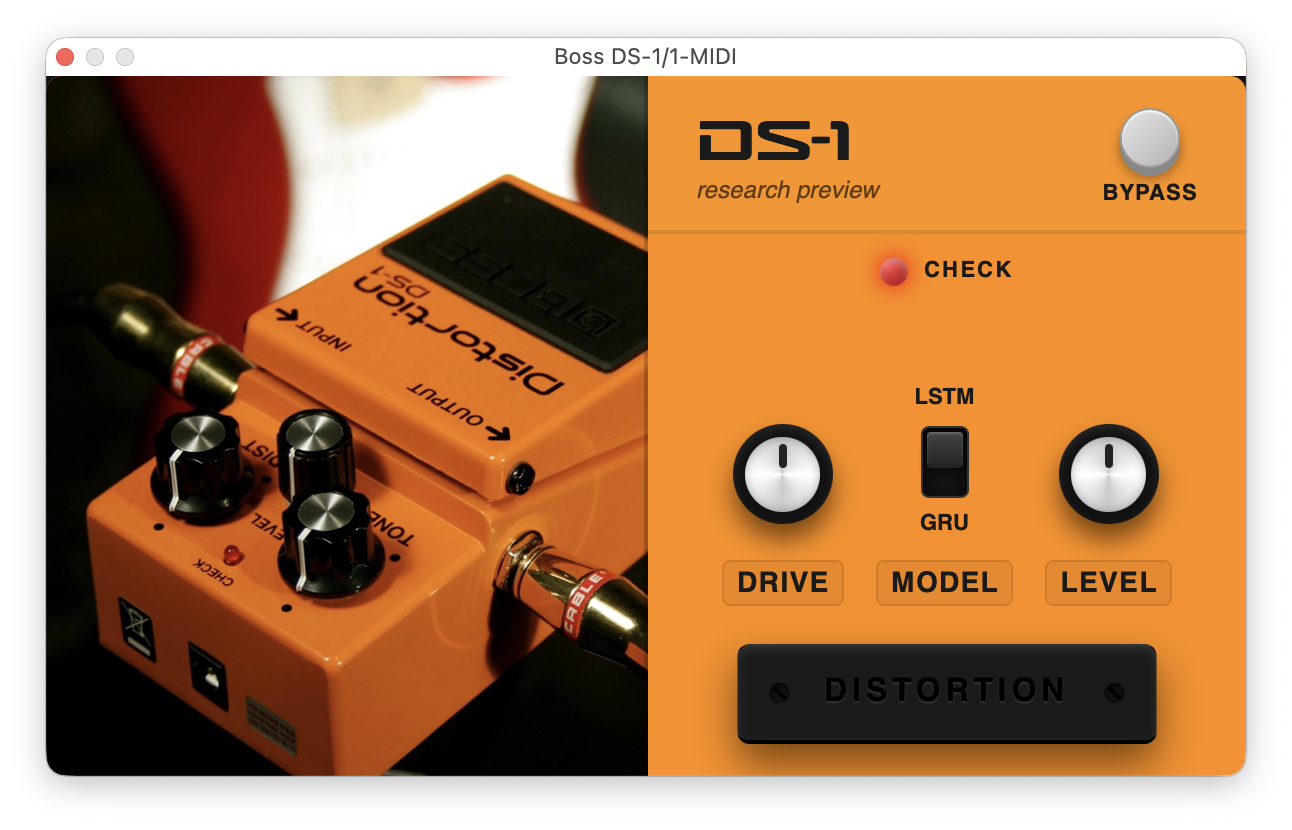
\includegraphics[width=0.9\textwidth]{images/plugin_ui.png}
  \caption[Plugin interface in Ableton Live]{The Boss DS-1 neural emulation plugin UI}
  \label{fig:plugin_screenshot}
\end{figure}
